% \Image{Capa do livro (; )}{PNLD2022-014-01.png}

% \Image{Ilustração do livro (Kalinka/David Shterenberg; Kalinka)}{PNLD2022-014-04.png}
% \Image{Ilustração do livro (Kalinka/David Shterenberg; Kalinka)}{PNLD2022-014-05.png}
% \Image{Ilustração do livro (Kalinka/David Shterenberg; Kalinka)}{PNLD2022-014-06.png}


\documentclass[11pt]{extarticle}
\usepackage{manualdoprofessor}
\usepackage{fichatecnica}
\usepackage{lipsum,media9}
\usepackage[justification=raggedright]{caption}
\usepackage[one]{bncc}
\usepackage[kalinka]{../edlab}
\usepackage{marginnote}
\usepackage{pdfpages}
\usepackage[printwatermark]{xwatermark}
\newwatermark[pagex=2]{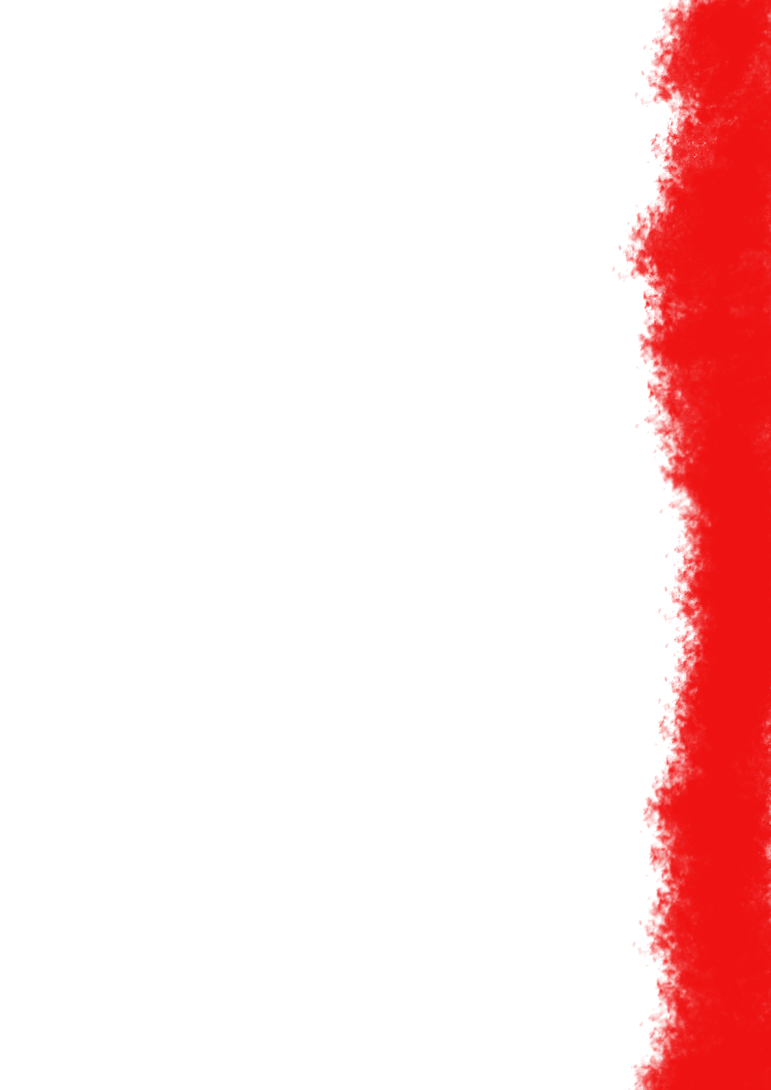
\includegraphics[scale=3.3]{watermarks/test-a.png}}	% página específica
%\newwatermark[oddpages]{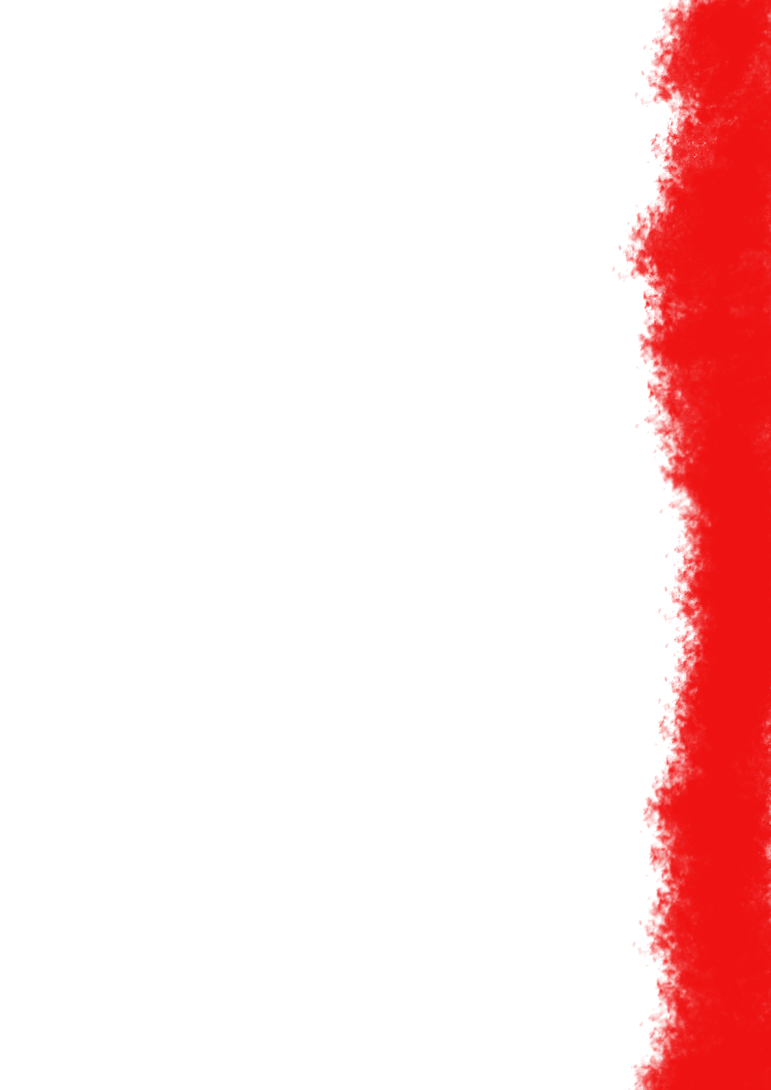
\includegraphics{watermarks/test-a.png}}			% páginas ímpars
%\newwatermark[evenpages]{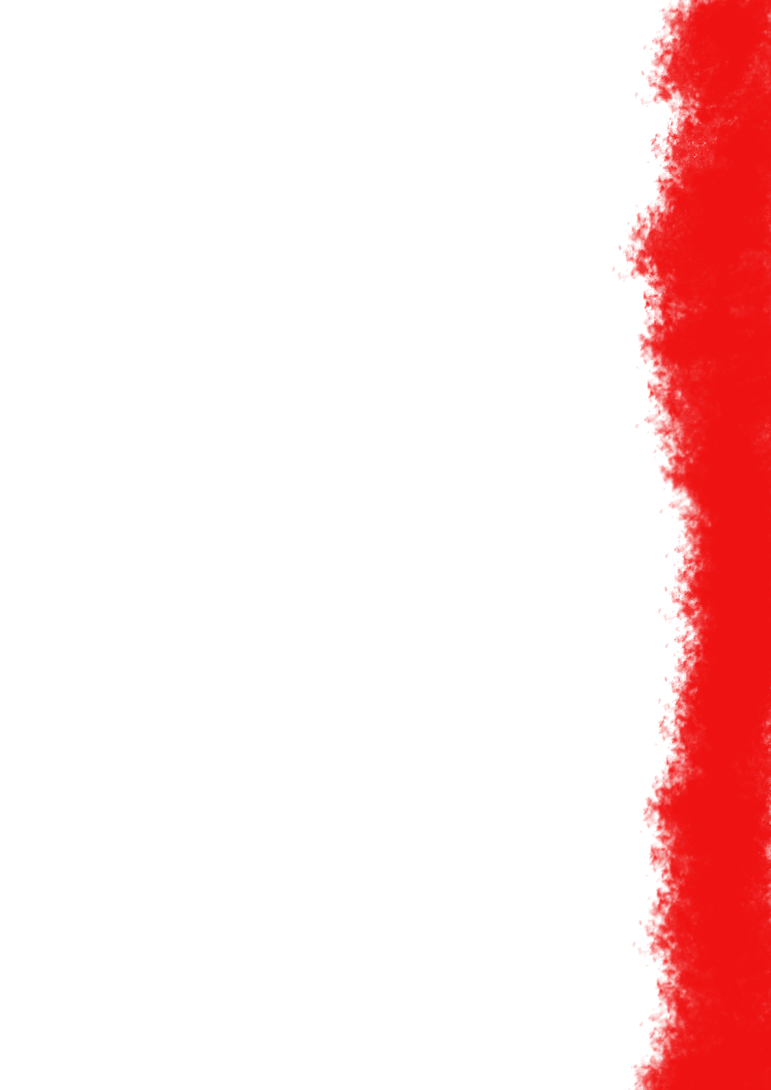
\includegraphics{watermarks/test-a.png}}			% págimas pares
\newwatermark[allpages]{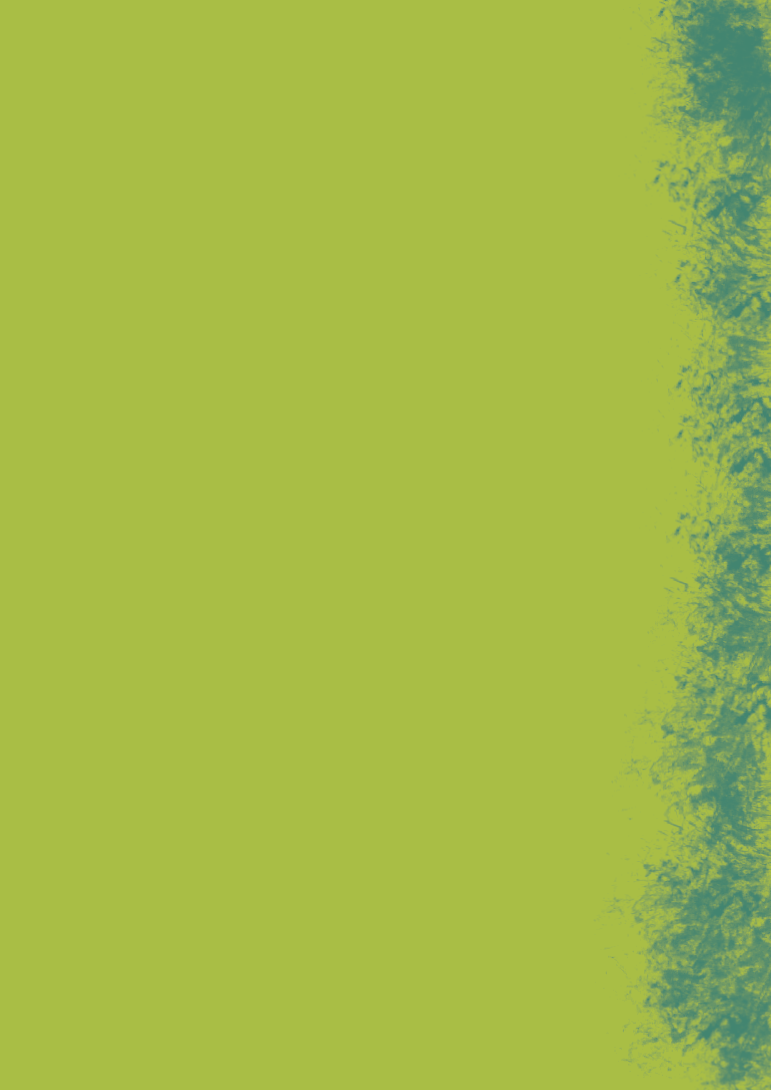
\includegraphics[scale=3.3]{watermarks/test-b.png}}

\pagecolor{cyan!0!magenta!10!yellow!28!black!28!}

\newcommand{\AutorLivro}{David Shterenberg}
\newcommand{\TituloLivro}{Louça}
\newcommand{\Tema}{Quotidiano de crianças nas escolas; nas famílias e nas comunidades (urbanas e rurais)}
\newcommand{\Genero}{Narrativos: fábulas originais; da literatura universal e da tradição popular; etc}
\newcommand{\imagemCapa}{./images/PNLD2022-014-01.png}
\newcommand{\issnppub}{978-65-86862-12-6}
\newcommand{\issnepub}{978-65-86862-11-9}
% \newcommand{\fichacatalografica}{PNLD0001-00.png}
\newcommand{\colaborador}{{Paulo Pompermaier e Renier Silva}}

\begin{document}

\title{\TituloLivro}
\author{\AutorLivro}
\def\authornotes{\colaborador}

\date{}
\maketitle

%\begin{abstract}\addcontentsline{toc}{section}{Carta ao professor}
%\pagebreak

\tableofcontents



\section{Sobre o livro}

%550 caracteres
\paragraph{O livro} \textit{Louça} (1930), do pintor russo David Shterenberg, traz uma série de naturezas-mortas para crianças com objetos familiares e cotidianos. As composições primorosas do livro convidam o pequeno leitor a interagir com o mundo onde vive e a explorar formas, cores e texturas. O ponto de partida do livro é um peixe em uma caçarola, cujo olho vê e observa tudo que há na cozinha: a mesa, copos, jarra, toalha, concha e outros utensílios de cozinha. A obra, assim, aborda objetos do cotidiano com um olhar artístico, utilizando-se do famoso tema das artes plásticas da natureza-morta para retratar objetos familiares ao cotidiano de qualquer criança.


%822 caracteres
\paragraph{Descrição} ``O olho do peixe tudo vê''. É esse enunciado que inicia a narração de \textit{Louça}. Nas páginas seguintes da obra, somos apresentados ao que é esse ``tudo'' que o olho do peixe vê: a mesa branca redonda, o copo alto amarelo, a toalha de mesa, a jarra pintada, a fruteira colorida com suas frutas, a concha funda vermelha, o ralador brilhante e outros objetos de cozinha. Cada objeto descrito é ilustrado com outros utensílios de cozinha que não estão enunciados, formando pequenos quadros que contextualizam o objeto presente na narração com outros elementos que compõem a cozinha da narrativa. As cores das ilustrações são ricas e vivas, aguçando a curiosidade e a imaginação, e as frases são muito curtas, permitindo uma maior compreensão da relação entre o signo gráfico e sua representação na ilustração. Todas as ilustrações reforçam as formas e geometrias, com linhas definidas que permitem a apropriação pelo aluno de conceitos básicos relacionados à forma dos objetos (o redondo da mesa, o retângulo do ralador, a meia-lua da fruteira, o quadrado da toalha etc.).

%411 caracteres
\paragraph{Competências} O livro \textit{Louça} permite o trabalho e desenvolvimento de diversas competências com a criança. Com frases curtas e ricas ilustrações, ele mostra as relações entre escrita e imagem. Incentiva o desenho, já que apresenta objetos criados por meio de formas elementares. Expõe a criança a diferentes manifestações artísticas (cor, forma, pintura, etc.), de modo que ela comece a desenvolver senso estético, além de apreender os diferentes atributos que constituem as formas e o espaço (alto, fundo, redondo, amassado etc.). Ao aguçar sua curiosidade pelo mundo, a obra ajuda a criança a reconhecer objetos simples do cotidiano, relacionando-os à sua experiência de leitura.

%862 caracteres
\paragraph{Aprofundamento} Este material tem a 
intenção de contribuir para que você consiga desenvolver um trabalho aprofundado 
com esta obra na sala de aula. Você encontrará informações sobre a autora, sobre 
o gênero e sobre os temas trabalhados ao longo do livro. Apresentaremos também 
algumas propostas de trabalho para a sala de aula que você poderá explorar livremente, 
da forma que considerar mais apropriada para os seus estudantes. Para a prática 
da Literacia Familiar, oferecemos um guia que pode ajudar nas orientações aos 
responsáveis pela criança, para incentivar o gosto pela leitura e contribuir para 
que os estudantes desenvolvam em casa habilidades que serão importantes no momento 
da alfabetização. Por fim, você encontrará sugestões de livros, artigos e sites 
selecionados para enriquecer a sua experiência de leitura e, 
consequentemente, a de seus estudantes.



\section{Sobre os autores}

\Image{Foto do autor e ilustrador (Kalinka; Kalinka)}{PNLD2022-014-02.png}

%532 caracteres
\paragraph{O autor} O pintor e artista gráfico David Shterenberg (1881-1948), de uma família judia humilde, nasceu em Jitómir, parte do império russo. Interessado por arte desde criança, em 1905 foi para Odessa em busca de formação e lá estudou fotografia. Em 1907, mudou-se para Paris е viveu em La Rouche (Montparnasse), residência de artistas pobres por onde passaram também pintores como Modigliani e Chagall. Na capital francesa, Shterenberg estudou na Academia de A. Vitti e participou de exposições em salões de pintura. A ambiência parisiense, que lhe deu a oportunidade de conviver com muitos artistas --- como o poeta Apollinaire ---, era marcada por experimentações artísticas e foi uma grande escola para o jovem pintor. 

Depois de dez anos, voltou para a Rússia, onde ocupou diversos cargos, como de Comissário de assuntos artísticos. Deu aulas no 	\textsc{vkhutemas} (Estúdios superiores de arte e de técnica), fundou o grupo \textsc{ost} (Sociedade dos pintores de cavalete) e organizou várias exposições, inclusive uma com Chagall, em Moscou (1922). 

As décadas de 1910 e 1920 marcam o amadurecimento do estilo de Shterenberg. Nessa época ele produziu uma série de naturezas-mortas que misturavam magistralmente elementos do cubismo e do primitivismo. Como notou o crítico de arte Iúri Guertchuk: “A natureza-morta exerceu um papel fundamental na cultura pictórica das primeiras décadas do século \textsc{xx}” e na trajetória de Shterenberg. Sem enveredar para o abstracionismo, representava objetos simples e rústicos que, com suas propriedades acentuadas, passam ao observador uma impressão táctil. Uma espécie de “naturalismo \textit{naïf}”, lembrando o trabalho do artesão. 

“A simplicidade surpreendente desses trabalhos é resultado de uma rigorosa seleção de procedimentos artísticos, do cálculo da composição com precisão matemática e do sucessivo afastamento de tudo o que é supérfluo. Por isso a linguagem pictórica lacônica de Shterenberg é tão ampla e flexível, rica em matizes emocionais, por isso ele conseguiu dizer tanto representando, numa tela vazia, apenas um copo com coalhada numa mesa oval de mármore ou um lúcio enorme em cima de um banquinho.”\footnote{Disponível em: \url{https://maslovka.org/modules.php?name=Content&pa=showpage&pid=141}.} 

\textit{Louça}, parte de uma série de livros ilustrados para crianças que Shterenberg criou entre 1928 e 1931, é uma amostra brilhante dessa fase do pintor e também um dos livros infantis russos publicados nas décadas de 1920 e 1930 que se tornaram objeto de colecionador. São publicações até hoje apreciadas, sendo parte de acervos de importantes museus e bibliotecas da Rússia, dos \textsc{eua} e da Europa.

%313 caracteres
\paragraph{A designer} Karina Aoki, nascida em São Paulo em 1977, é formada em Arquitetura e Urbanismo pela \textsc{fau-usp}. Atuou como diretora de arte e coordenadora de estúdio da São Paulo Criação -- Rafic Farah durante oito anos, atendendo clientes como Mitsubishi Motors do Brasil, Fundação Roberto Marinho, Fast Shop, Casa do Saber, Escola da Cidade, Museu de Arte Brasileira da \textsc{faap}, restaurantes Arabia, Spot e Ritz, marcas de moda Maria Bonita, Mandi, Lucy in the Sky e
Brooksfield Donna, cinema \textsc{hsbc}/Belas Artes, e o designer Carlos Motta. Foi também editora de arte da revista Casa Vogue (Edições Globo Condé Nast) por seis anos e supervisora de arte do departamento de literatura da editora \textsc{ftd} Educação, sendo responsável por cerca de 70 títulos. Atualmente desenvolve projetos independentes nas áreas de identidade visual, embalagem, expografia e editorial.

Karina Aoki adaptou a capa de modo que a criança brasileira tivesse acesso ao
desenho original. Todas as ilustrações originais foram tratadas, com atenção à cor, ao traçado e ao tratamento dado pelo pintor.

%358 caracteres
\paragraph{A tradutora} 
Daniela Mountian graduou-se em História pela Universidade de São Paulo (\textsc{usp}), mestrado sobre Fiódor Sologub, expoente do simbolismo russo, e doutorado-sanduíche sobre o vanguardista Daniil Kharms, com estágio de um ano no Instituto de Literatura Russa da Academia Russa de Ciências (Casa de Púchkin), em São Petersburgo. Atualmente, pesquisando a literatura infantil russa e brasileira dos anos 1920 e 1930, é pós-doutoranda (\textsc{dtllc/usp}) com apoio da Fundação de Amparo à Pesquisa do Estado de São Paulo (\textsc{fapesp}, processo nº 2017/24139-9), também com um ano de estágio na Casa de Púchkin. É criadora e editora-chefe da Kalinka, dedicada à literatura russa. Foi indicada ao prêmio Jabuti pela tradução de \textit{“Os sonhos teus vão acabar contigo”: prosa, poesia, teatro}, de Daniil Kharms (Kalinka, 2013, com Aurora Bernardini e Moissei Mountian). Traduziu com seu pai, Moissei, o conto “Luz e sombras”, de Sologub, para a \textit{Nova antologia do conto russo} (Editora 34, 2011), e “Ivan Fiódorovitch Chponka e sua titia”, de Nikolai Gógol, para a \textit{Antologia do humor russo} (Editora 34, 2018); e os livros \textit{Diário de um escritor (1873): Meia carta de “um sujeito”}, de Fiódor Dostoiévski (Hedra, 2016), e \textit{A ressurreição do lariço} (Contos de Kolimá 5), de Varlam Chalámov (Editora 34, 2016). Prefaciou e organizou a antologia \textit{Contos russos juvenis} (Kalinka, 2021).
 
Daniela Mountian adaptou as ilustrações de Shterenberg em frases simples e sonoras. Cada oração evidencia um objeto e incentiva a criança a buscar outros elementos na composição.

\section{Sobre o gênero}

%55 caracteres
\paragraph{O gênero} O gênero deste livro é \textit{narrativa}. 

\Image{O gênero da narrativa proporciona ao leitor uma abertura ao mundo. (Pixabay/Tumisu; CC-BY-2.0)}{PNLD2022-014-07.png}

%596 caracteres
\paragraph{Descrição} Em sua base, pode-se definir a narrativa como um gênero que conta uma história, normalmente em estrutura linear, ou seja, começo, meio e fim, e com personagens. 
Dentre os tipos de narrativas mais comuns na literatura infantil, estão: mito, lenda, 
fábula e apólogo. Nos livros infantis, as possibilidades narrativas são quase ilimitadas, pois quase tudo pode integrar a narrativa e fazer parte dela como personagem, já que a capacidade reflexiva das crianças nesta idade ainda está em um nível primário. No caso de \textit{Louça}, por exemplo, o impulso narrativo parte do olho de um peixe, que vai observar os elementos cotidianos e, assim, estruturar o encadeamento da narrativa.

%603 caracteres
\paragraph{Interação} As narrativas são uma forma de inserir os sujeitos no mundo. 
São elas que apresentam boa parte dos valores culturais da sociedade 
onde se vive. Mas não é só passivo o papel das crianças nesta experiência. 
As interações entre dois ou mais personagens onde se verifica
uma ação de linguagem organiza e impulsiona experiências compartilhadas,
importantes para o desenvolvimento psíquico do sujeito nos primeiros anos de vida.
Neste sentido, as narrativas são uma ótima ferramenta para
apresentar o mundo e capacitar as crianças para viver nele, mas como se
trata de um trabalho com a linguagem, sempre dando espaço à individualidade, 
seja na compreensão das histórias, na identificação com as personagens, ou 
no ato de narrar.

%862 caracteres
\paragraph{Competências} 
Através de elementos dos mitos, contos e histórias da cultura local e internacional, desenvolve-se a sensibilidade narrativa e a capacidade de imaginação das crianças. Para um bom desenvolvimento da capacidade narrativa e imaginativa é necessária a intermediação do educador, que vai trazer novos olhares, análises e discussões para ajudar a criança na construção do significado. Essas são etapas fundamentais para o desenvolvimento linguístico e a aquisição das competências de leitura e escrita. Por meio da narrativa, inclusive, a criança passa do diálogo ao monólogo, pois passa a ser capaz de elaborar um discurso para si com maior autonomia, sem a intermediação necessário no diálogo.
O conjunto de elementos verbais e visuais da narrativa proporcionam, assim,
uma abertura ao mundo e um convite para integrá-lo pela curiosidade e pela imaginação.


\section{Temas}

\subsection{Quotidiano de crianças nas escolas; nas famílias e nas comunidades (urbanas e rurais)}

%136 caracteres
\paragraph{Abordagem} Toda a narração centra-se em elementos do quotidiano da criança, trazendo objetos presentes nas cozinhas e casas: copos, mesas, toalhas, pratos, jarros, conchas etc.

%206 caracteres
\paragraph{Descrição} O livro oferece uma ótima oportunidade de explorar 
e aprofundar a relação da criança com objetos do cotidiano, demonstrando a relação entre as palavras e as coisas através de um olhar artístico e criativo. A representação artística de objetos cotidianos, ademais, estimula a imaginação da criança e sua identificação com a história narrada.

%275 caracteres
\paragraph{Competências} Este tema relaciona-se, principalmente, ao 
campo da experiência Espaços, tempos, quantidades, relações e transformações
descrito pela \textsc{bncc}, que explora a curiosidade infantil sobre o mundo 
para proporcionar a construção de conhecimento a partir da observação e exploração.
Também pode ser relacionado ao campo da experiência Traços, sons, cores e formas, pois estimula a apreensão da criança de elementos relacionados às cores e formas que caracterizam os objetos quotidianos.


\section{Modelagem de aula}
A seguir você encontrará a descrição de uma aula modelo como exemplo 
prático de exploração do livro com estudantes. Esta seção apresentará 
orientações sobre como organizar a sala de aula para receber os 
estudantes, exercitar a interação verbal e prepará-los para o 
momento da leitura.

Em seguida, você encontrará a \textbf{Leitura dialogada}, um 
tópico destinado a te orientar para o momento específico da 
leitura com os estudantes. Por fim, no tópico 
\textbf{Propostas de atividades}, você encontrará ideias 
de práticas que pode explorar com as crianças em sala de 
aula antes, após e durante a leitura. 

Essas atividades podem ser trabalhadas de acordo com a 
disponibilidade do seu cronograma. Fique à vontade para adaptá-las 
da forma que achar melhor para os seus estudantes. Cada turma é única 
e o seu conhecimento prático das características de cada aluno será 
essencial para definir a melhor forma de aplicar essas ideias. 

O objetivo deste manual é oferecer algumas ideias 
e inspirações para um trabalho que pode ser desenvolvido tanto 
a curto, quanto a médio e longo prazo. Sinta-se à vontade para 
personalizar a aula e torná-la sua, aplicando seus conhecimentos, sua 
personalidade e aproveite para fortalecer 
seu vínculo com a turma.


\subsection{Antes de ler}

\BNCC{EI02EO03}
\BNCC{EI02EO04}
\BNCC{EI02CG01}
\BNCC{EI02ET01}
\BNCC{EI02ET05}

%Alterar o nível escolar nesse parágrafo.
Como este trabalho será realizado com crianças da \textbf{Creche 2}, 
que ainda não têm tanta intimidade com o livro enquanto objeto, você terá o 
papel essencial de mediar este contato. 

Nosso objetivo é que os próprios estudantes possam manusear 
e explorar o livro de forma autônoma, mas, para que isto aconteça, você 
pode ajudar a tornar o caminho mais convidativo com atividades que tenham 
intencionalidade educativa. 

A \textsc{bncc} define intencionalidade educativa como ``organização 
e proposição, pelo educador, de experiências que permitam às crianças 
conhecer a si e ao outro e de conhecer e compreender as relações com a 
natureza, com a cultura e com a produção científica, que se traduzem nas 
práticas de cuidados pessoais (alimentar-se, vestir-se, higienizar-se), 
nas brincadeiras, nas experimentações com materiais 
variados, na aproximação com a literatura e no encontro com as 
pessoas''.\footnote{\textsc{bncc}, página 39}

É importante manter essa intencionalidade em mente não apenas na condução 
das atividades propostas neste manual, mas também para aproveitar as 
oportunidades espontâneas de construir conhecimentos que podem surgir durante 
a interação direta com os estudantes.

\begin{enumerate}
%836 caracteres
\item \textbf{O ambiente}\quad Antes de iniciar o trabalho com o livro, é importante que você 
prepare o ambiente para receber a turma. Como o trabalho com o livro terá 
três momentos (antes, durante e depois da leitura), seria interessante que você 
criasse um ambiente para cada etapa. Nas \textbf{Sugestões de referências complementares} 
você encontrará um artigo que discorre sobre a importância da organização da sala 
de aula para a educação infantil, que pode ser um bom guia para a criação desses 
ambientes.
Para o momento antes da leitura, sugerimos uma atividade que estimule a
associação entre  objetos do cotidiano das crianças e as imagens contidas no livro. Será necessário comunicar os pais antecipadamente para separarem alguns objetos e utensílios do quotidiano da criança para levarem à escola: colher, copo, prato, potes e travessas de plástico. Deixe, se possível, alguns desses objetos separados para o caso de alguma criança não trazer. A atividade pode ser desenvolvida em sala de aula ou na biblioteca.

\Image{As crianças vão levar utensílios de plástico para observarem em aula as diferenças de cor, tamanho, formas etc. (Piqsels; Domínio público)}{PNLD2022-014-09.png}


%413 caracteres
\item \textbf{Materiais}\quad Talheres e utensílios de cozinha de plástico; folha sulfite A4; lápis de cor.

%632 caracteres
\item \textbf{Desenvolvimento}\quad O professor explicará, com uma semana de antecedência, que os alunos devem trazer uma colher, copo ou prato para a aula (importante serem de plástico, ou outro material que não apresente perigos à integridade física da criança). No dia da atividade, o educador convidará os alunos para observar quais as diferenças entre os seus materiais e os dos colegas, propondo que percebam as diferenças de cor, forma, material,  tamanho etc. Prepare um local de registro com esses tópicos e o nome dos alunos, para anotar as respostas. Facilite a comunicação entre as crianças mediando os diálogos e fomentando-os a trocar informações sobre as características dos materiais. Pode, igualmente, ser trabalhado o cuidado e atenção com esses utensílios, que serão devolvidos aos familiares.

\item \textbf{Perguntas para avaliar}\quad As crianças interagiram e se interessaram pelos materiais dos colegas? Conseguiram perceber as diferenças? E as semelhanças? Elas já conseguem diferenciar cores, formas, materiais e tamanho? Se não, como estimular a aquisição dessas habilidades? 

\end{enumerate}


\subsubsection{A interação verbal} 
Criar situações em que as crianças precisam dialogar diretamente com 
você é uma das práticas mais importantes de Literacia, pois elas estimulam 
o desenvolvimento linguístico, ampliam o vocabulário e reforçam a 
capacidade dos estudantes de compreenderem o que ouvem e se expressarem 
pela fala. O diálogo livre com a criança também reforça sua autoestima, pois 
a faz se sentir ouvida e valorizada pelo adulto, ao vê-lo prestar atenção 
no que ela tem a dizer. Portanto, sempre que possível, reserve um tempo na 
aula apenas para a interação verbal. 

Como esse tipo de interação é espontânea e intimamente atrelada ao 
desenvolvimento de cada estudante, nossas orientações não serão específicas. 
A ideia é que você adapte este momento de acordo com as respostas e os 
repertórios das crianças. É um momento de estreitamento de vínculos e, portanto, 
fique à vontade para ser espontânea e para explorar os tópicos que achar 
mais interessantes para a sua turma.

Inicie as conversas com naturalidade, seguindo os objetos de atenção das crianças. 
Você pode partir de objetos que estejam analisando
para iniciar um assunto e incentivar que se expressem. Ainda que a
criança não fale corretamente, continue interagindo, 
pois a intenção aqui é que a criança perceba que outras pessoas estão respondendo 
à sua comunicação. 

Fique atento a todas as formas de expressão: os gestos, as falas, as 
expressões faciais, para onde olham\ldots{} tudo pode ser explorado durante a conversa. 
Demonstre curiosidade sobre eles, seja um ouvinte entusiasmado e incentive que eles 
conversem entre si. Faça perguntas e construa a resposta junto com as crianças. 

A seguir, algumas dicas que podem contribuir para que a interação verbal 
seja produtiva em sua sala de aula: 

\begin{enumerate}
\item Sente-se no chão e brinque com eles, estabelecendo 
contato visual. Além das pequenas frases que conseguem formar, vocalizações, 
gestos e expressões faciais podem ser boas formas de comunicar.

\item Não se esqueça que a conversa é uma troca e, portanto, 
evite ficar falando sozinho ou desvalorizar as respostas das 
crianças quando não conseguem formular frases completamente articuladas. 
Nunca descarte uma tentativa de comunicação. 

\item Evite utilizar falas negativas que desencorajam o diálogo. 
Se precisar que a turma 
corrija algum comportamento, explique claramente a razão e 
oriente com calma. Incentive positivamente as crianças e 
destaque o motivo de seus elogios. 

\item Aproveite alguns momentos durante a conversa para chamar 
a atenção das crianças para os sons das palavras e das letras que você 
acabou de usar ou que eles pronunciaram.  

\item Fale sempre com as crianças, pois, apesar de alguns estarem começando a falar,
são capazes de compreender muito.

\item Explore possibilidades de interação como apontar e 
nomear objetos, pessoas e animais, imitar a criança ou pedir que 
ela o imite, fazer caretas, reproduzir sons de 
animais para que repitam, ensinar os nomes de partes do corpo, 
entre outras atitudes que estimulem a comunicação com a criança. 

\item Muitas dessas dicas poderão ser aproveitadas pela 
família durante a prática da Literacia Familiar. Portanto, 
se achar necessário, compartilhe algumas destas orientações 
com as famílias dos estudantes.
\end{enumerate}


\subsection{A leitura dialogada}
Este é o momento em que será realizada a leitura propriamente dita. 
Se possível, crie um \textit{cantinho da leitura} em sua sala de aula. Um 
ambiente confortável, de preferência em que todos se sentem no chão ou 
em pufes para que consigam enxergar as ilustrações do livro que está 
sendo lido e interagir com facilidade. Se houver possibilidade, mantenha 
sempre os livros da turma em uma altura da estante que permita fácil 
acesso para os estudantes ou guarde os livros em uma caixa que as crianças 
possam mexer com autonomia. É importante que elas tenham autonomia para 
acessar os livros e se sintam à vontade para pegá-los sempre que quiserem. 

\Image{É importante que o cantinho da leitura proporcione autonomia para as crianças. (Elza Fiúza/ Agência Brasil; CC BY-NC 2.0)}{PNLD2022-014-08.png}

Outra possibilidade de ambiente para esta leitura, se a escola permitir, 
é efetuar essa leitura ao ar livre, embaixo de uma árvore, onde as crianças 
possam ouvir os sons dos pássaros e sentir o cheiro da grama. Sair da sala 
de aula pode oferecer um ótimo leque de experiências aos seus estudantes e 
reforçar a conexão entre a natureza do livro e a realidade.  

Reserve uma boa parte da aula para o momento da leitura com os estudantes, 
pois é importante que esse momento aconteça sem pressa. O objetivo da 
leitura dialogada é que seja uma leitura em bate-papo. A criança deve 
assumir um papel ativo na leitura, mesmo que ainda não seja capaz de 
ler sozinha. Além de promover o gosto pela leitura, esta prática estimula 
o desenvolvimento da linguagem, enriquece o vocabulário e 
aumenta o conhecimento de mundo.

%Especificar o livro.
No caso de \textit{Louça} o diálogo durante a leitura é 
ainda mais importante, pois isso permite que os alunos comecem a associar as palavras às suas representações imagéticas, além de aprofundar a percepção dos estudantes sobre os diversos aspectos e características que constituem os objetos ilustrados na obra.
Você deve interagir com eles durante toda a 
leitura, fazendo perguntas e partindo de detalhes do livro para 
levantar novas questões. 

A seguir, algumas orientações para aproveitar este momento e desenvolver uma atividade durante a leitura: 

\begin{enumerate}
%177 caracteres
\item \textbf{Contexto}\quad Após a atividade anterior à leitura, as crianças já 
começaram a perceber os objetos domésticos e a observar suas diferentes características, o que vai aguçar e facilitar seu mergulho na obra. O objetivo desta atividade é
trabalhar a abstração e proporcionar a rica associação entre o material literário e o cotidiano. A atividade pode ser desenvolvida em sala de aula, biblioteca ou em um espaço externo.

\item \textbf{Materiais}\quad Livro \textit{Louça}; materiais que os alunos levaram de suas casas para a sala de aula.


\item \textbf{Desenvolvimento}\quad Nesta atividade, propõe-se que os alunos façam comparações entre os materiais que trouxeram para sala com as imagens contidas no livro.
O educador poderá juntar duas mesas e colocar alguns dos utensílios trazidos pelas crianças, para que, durante a leitura e na apresentação das imagens do livro, possam pegar e manusear os objetos que acharem parecidos com os que estão sendo apresentados em \textit{Louça}. Ao permitir que se movimentem livremente e criem suas associações entre os objetos e a obra, a leitura se torna mais dinâmica e divertida. Durante a leitura, estimule o diálogo depois de ler as frases do livro. Peça para que os alunos percebam os detalhes das imagens e dos objetos, estimulando o senso estético. Auxilie os menores e solicite a ajuda dos maiores. 
 
%230 caracteres
\item \textbf{Manuseio}\quad Deixe que as crianças manuseiem o livro 
e explore com elas todos os elementos que o compõem. Mostre o que é a 
capa e onde estão as páginas. Deixei também que manuseiem livremente os objetos de casa, percebendo as diferentes texturas e formas de manusear cada coisa.

%495 caracteres
\item \textbf{Diálogo}\quad Como os objetos da narrativa são parte da realidade social das crianças, o livro permite muitas pontes de diálogo, que associem a história narrada à vida das crianças.
É interessante convidar as crianças a partilharem suas experiências com os objetos apresentados, perguntando quais objetos da obra eles conhecem e quais desconheciam. Relacione os objetos comentados e manipulados pelos alunos com aqueles apresentados pelo livro.

%346 caracteres
\item \textbf{Escuta}\quad Elogie atitudes positivas, como 
a boa interação com a história lida e a solicitação de interagirem com ela. Se os estudantes tentarem 
tomar o seu lugar e começar a falar sobre a história ou sobre os objetos, valorize e escute com atenção o que estiverem falando. Mas não 
force a leitura. Se as crianças estiverem cansadas, faça outra atividade 
e retorne depois. 

%935 caracteres
\item \textbf{Leitura}\quad Faça perguntas e comentários que aumentem o 
interesse e aticem a curiosidade das crianças sobre a história. Faça 
uma leitura devagar, apresentando o nome dos objetos, suas funções e suas diferentes características.
Faça perguntas que realcem as diversas dimensões do objeto:

\begin{itemize}
\item Qual a cor dessa chaleira?
\item Essa mesa é redonda ou quadrada?
\item Qual objeto é mais fundo?
\item O copo é mais alto que a xícara?
\end{itemize}

Explore as diversas dimensões do espaço com as crianças.
Se elas não souberem responder, explique o que significa cada uma dessas dimensões.
Com os objetos trazidos de casa, essa associação fica ainda mais fácil, pois pode-se mostrar essas diferenciações na prática, comparando o tamanho, a profundidade e a cor dos objetos.
No manuseio do livro, não tenha pressa em passar as páginas. Deixe que os estudantes 
observem as ilustrações e as palavras, dê tempo para que construam suas imagens 
mentais a partir da história que foi lida e das ilustrações presentes na página. 

Ao explorar a leitura, dê emoção 
à narrativa. Enfatize as palavras desconhecidas,
capriche nas expressões faciais e traga, ao final, comentários sobre os objetos ilustrados.
Deixe-se guiar pela atenção das crianças, mas se perceber que 
elas estão dispersas ou saltando aleatoriamente as páginas, ajude-as 
a retornar à história. Crie um ambiente amigável onde a criança 
se sinta à vontade para fazer perguntas e comentários durante a leitura.

%382 caracteres
\item \textbf{Interação}\quad Reforce a relação entre as palavras e as ilustrações 
do livro, apontando para elas com o dedo. Destaque os sons de algumas 
palavras mais difíceis. Interrompa a leitura em alguns momentos e peça que 
os estudantes repitam palavras e as sentenças do livro. Se possível, 
releia a mesma história outras vezes ou explore as páginas em uma ordem 
diferente, começando, por exemplo, pelos últimos objetos apresentados e finalizando com o peixe que tudo vê.

\item \textbf{Perguntas para avaliar}\quad As crianças conseguiram realizar a atividade? As menores exploraram a proposta sensorialmente? As maiores interagiram com as menores, ajudando-as a realizar o proposto? Como foi a comunicação verbal das menores? E a corporal? 
\end{enumerate}


\subsection{Propostas de atividades}

\BNCC{EI02TS02}
\BNCC{EI02CG02}
\BNCC{EI02EF01}
\BNCC{EI02EF03}
\BNCC{EI02ET01}
\BNCC{EI02ET05}

\begin{enumerate}
%700 caracteres
\item \textbf{Contexto}\quad A sugestão de atividade pós-leitura tem como objetivo trabalhar o desenvolvimento da motricidade e a percepção da ação como capacitadora de transformação de elementos. A ideia é proporcionar que as crianças tentem reproduzir em argila e/ou massinha as formas dos objetos que trouxeram para sala, com o auxílio e participação ativa do professor.

\Image{O professor irá escolher alguns objetos para os alunos reproduzirem com argila ou massinha. (Pixabay; CC-BY-2.0)}{PNLD2022-014-10.png}

\item \textbf{Materiais}\quad Argila ou massinha.

%650 caracteres
\item \textbf{O ambiente}\quad Sala de aula ou espaço externo.

%950 caracteres
\item \textbf{A atividade}\quad O professor escolherá alguns objetos para os alunos reproduzirem com massinha ou argila. O nível de complexidade deve ser definido para cada idade. Oriente e ajude as crianças no desenvolvimento da atividade, indicando como movimentar as mãos para reproduzir o objeto. Não é necessário ser em tamanho fiel nem igual, pois a ideia é potencializar o processo e a ação. Faça com que a atividade seja prazerosa e divertida. Divida os objetos em subgrupos e proporcione uma atividade coletiva mais organizada. Após a confecção dos objetos, estabeleça um diálogo entre as esculturas e as ilustrações do livro. Pergunte quais são as semelhanças e as diferenças: pode-se explorar as aproximações entre cores, funções, diferentes tamanhos, profundidades etc. Indague as crianças sobre o que elas tentaram representar, reforçando a associação entre a palavra e a coisa.


%550 caracteres
\item \textbf{Interação}\quad Após a brincadeira de modelar, pode-se voltar ao livro para ver se os estudantes aprofundaram sua capacidade de reconhecer as cores e formas do livro.
Deixe que o livro seja manipulado pelos estudantes. Incentive que eles tentem repetir o nome dos objetos e suas características,
faça perguntas e proponha que imaginem juntos outros objetos e suas funções.
Quando as crianças propuserem suas ideias, interaja com o pensado e apresentado pelas crianças, fazendo perguntas que as auxiliem a desenvolver o pensamento iniciado.

\item \textbf{Perguntas para avaliar}\quad A turma se engajou no proposto? Como se comportaram? Ficaram curiosos com o tema? As crianças menores tentaram imitar os movimentos das maiores? 
\end{enumerate}


\section{Literacia familiar}
O \textsc{pna} dá destaque especial para a importância do envolvimento da família 
no processo pedagógico nesta faixa etária e denomina Literacia Familiar o conjunto 
de experiências e práticas relacionadas à linguagem (oral, escrita ou lida) vivenciadas 
com os cuidadores. 

Essas estratégias podem começar a ser colocadas em prática desde a 
gestação e continuar até o final da adolescência. São práticas simples e divertidas 
que estimulam o desenvolvimento de quatro atividades fundamentais: ouvir, falar, 
ler e escrever que criam momentos de afeto e interação para a família. 

Para que esse trabalho conjunto entre escola e família funcione, é 
fundamental que a escola esteja em constante diálogo com os responsáveis e 
você consiga orientá-los. Um grupo em aplicativos de mensagens instantâneas ou um 
grupo de e-mails são saídas viáveis para que a comunicação se estabeleça e pode ser 
uma forma útil das famílias compartilharem suas vivências e trocarem sugestões 
de abordagens, sempre contando com a sua mediação. 

Com o objetivo de incentivar 
a prática da \textit{literacia familiar}, se possível, organize um rodízio entre os familiares 
das crianças para emprestar o livro da biblioteca da turma. Neste caso, crie um caderno 
de registro e estabeleça períodos para cada família ficar com o livro. É importante 
que os familiares compreendam a seriedade deste compromisso, pois o livro pertence 
ao acervo da sala e, portanto, deve ser bem cuidado e devolvido na data acordada. 

Se não for possível garantir o acesso direto dos cuidadores da criança ao livro, 
grave um vídeo direcionado a eles, contando a história e apresentando algumas 
das ilustrações. O importante é que os familiares saibam com clareza qual livro 
está sendo trabalhado, a história contada e se sinta seguro para explorar as temáticas 
do livro com a criança. Orientações claras e a manutenção do canal de comunicação com 
os responsáveis é essencial para que eles se sintam seguros e à vontade para fazer perguntas 
se tiverem dúvidas. 

Neste manual, você encontrará algumas práticas que podem ser 
recomendadas aos familiares para ajudá-los a expandir e aprofundar o trabalho 
que você iniciou em sala de aula.


\subsection{Importância da leitura}
Na escola, aprendemos a ler letras, mas é importante ter em mente que nós 
lemos o mundo desde muito pequenos: “lemos” os animais que passam pelos nossos 
quintais, a expressão no rosto dos nossos familiares, as cores que pintam o céu 
em um fim de tarde. 

Vamos aprendendo, ao longo da vida, a interpretar acontecimentos 
e sons que escutamos e a utilizá-los para nossa comunicação. Aprender a ler textos e 
escrevê-los expande a nossa leitura do mundo, pois permite que sejamos capazes de 
interpretar um código e experimentar, a partir dele, novas experiências e conhecimentos. 

O simples contato com os livros já permite um leque grande de sensações: 
sentimos as texturas, as formas, vemos as cores do livro, escutamos o som da página 
virando e o som da voz do narrador, se a história estiver sendo lida em voz alta. Para uma 
criança pequena, são experiências que podem contribuir diretamente com o desenvolvimento psicomotor 
e cognitivo. 

Nosso papel, enquanto mediadores de leitura, é contribuir para que essas 
sensações sejam associadas a momentos positivos, de construção de 
conhecimento e exercício de imaginação. 

Com os livros, podemos conhecer mais da história humana, descobrir informações 
novas sobre sociedades diferentes da nossa, imaginar situações e contextos inéditos 
para nós e aumentar o nosso repertório. São por meio deles que melhoramos nossa 
capacidade de interpretação, de expressão, de análise e senso crítico. Boas habilidades 
leitoras podem contribuir para o desenvolvimento de um estudante em todas as outras 
disciplinas, pois exercem influência direta na forma como absorvemos e 
construímos conhecimento.


\subsection{O papel da família na formação do leitor}
A família é peça fundamental na formação do leitor, pois é ela quem primeiro 
ensina a criança a ler. Não apenas os textos escritos, mas a ler o mundo, a 
interpretar os estímulos que a cercam, a construir seu próprio vocabulário e a 
comunicar seus pensamentos e necessidades. Na fase em que estão, os bebês 
absorvem o conhecimento com voracidade e tentam aprender a se comunicar. 

O universo das letras é muito presente na vida das crianças antes mesmo de sua 
entrada na escola. Aparece nas histórias e ilustrações do livro que o cuidador 
lê ao colocá-la para dormir, nas situações em que vê os responsáveis se comunicarem 
pela escrita ou nos textos que podem permear seu cotidiano (nos outdoors, na 
televisão, no celular, manuais de instrução entre outros). 

Os familiares têm, 
portanto, uma ótima oportunidade de apresentar a leitura com leveza, de forma 
prazerosa, associado ao contexto em que a criança vive e à momentos de diversão. 
Você poderá orientar os pais nesta tarefa, ensinando-os com este guia a aproveitar 
as oportunidades para trabalhar a Literacia com a criança.


\subsubsection{Práticas de literacia familiar} 

São muitas as experiências que a prática da \textit{literacia familiar} 
pode oferecer às crianças. A seguir, explicamos cada uma delas para que você possa, 
se achar necessário, compartilhar com os responsáveis enquanto estiver orientando-os: 

\paragraph{Interação verbal} Aumentar a quantidade de conversas com as 
crianças, fazendo perguntas para incentivar o diálogo.

\paragraph{Leitura dialogada} Interagir com a criança durante a leitura 
em voz alta, criar expectativa sobre o livro, chamar a atenção para detalhes 
das ilustrações e comentar o enredo.

\paragraph{Narração de histórias} Interagir com a criança enquanto 
estiver narrando uma história, por exemplo, incluindo-a na ação, utilizando 
marionetes ou permitindo que ela complete a narrativa.

\paragraph{Contatos com a escrita} Apresentar as letras para as 
crianças, incentivar que tentem escrever ou ler, ajudá-los a desenhar letras, 
entre outras formas de incentivar o contato com as palavras.

\paragraph{Atividades diversas} Qualquer atividade com a criança 
pode ser utilizada para contribuir para a alfabetização. Jogos, brincadeiras, 
instrumentos musicais, canto, dança, passeios e viagens oferecem boas 
oportunidades de aprendizado.

\paragraph{Motivação} Atitudes que motivem as crianças à envolver-se com 
o mundo da leitura e da escrita.

\subsection{Exercitando a literacia familiar}

\BNCC{EI02EF03}
\BNCC{EI02EF04}
\BNCC{EI02ET01}
\BNCC{EI02EO03}
\BNCC{EI02EO04}

\begin{enumerate}
%700 caracteres
\item \textbf{Como começar}\quad O contato da família com a criança e o livro começam desde a primeira atividade proposta. Os pais devem ser convidados para auxiliar as crianças na escolha dos objetos para trazer no dia da atividade. Peça para que, no processo de escolha, ajudem a criança a refletir sobre os aspectos do material que serão trabalhados em sala: cor, forma, dimensões etc. Eles podem, igualmente, relacionar os objetos e suas características aos usos cotidianos, reforçando as ligações entre a obra e o cotidiano da criança.
Essa é uma forma de iniciar o contato dos pais com as crianças na leitura, pois os envolve nas atividades que serão desenvolvidas em sala de aula.

%650 caracteres
\item \textbf{Leitura}\quad A família pode continuar 
explorando os temas apresentados pelo livro. Uma das formas de fazer isso é solicitar aos pais que conversem com a criança sobre os diferentes aspectos acerca do mundo ao seu redor e a percepção da criança sobre eles: dia, noite, manhã, tarde, dentro, fora, cheio, vazio, seco, molhado, alto, baixo, fundo, raso, redondo, quadrado, amassado, liso, brilhante, fosco etc. São noções de espaço, tempo, forma e aspecto desenvolvidos no livro que, ao serem abordados no cotidiano da criança, aumentam a percepção do estudante sobre a obra e tornam o processo de leitura lúdico e divertido. Assim, envolve-se a família com a narrativa do livro e as atividades desdobradas e exploradas em sala de aula.
Outra possibilidade, quando a família tem acesso ao livro, é ler alguns trechos com a criança em um horário estipulado para isso. A leitura em família é importante pois relaciona o ato de ler e manusear um livro com o campo de suas experiências afetivas.

%1073 caracteres
\item \textbf{Instrução}\quad Informe aos pais sobre a estrutura do livro e as principais competências desenvolvidas em sala de aula.
Oriente-os a, quando possível, ler alguns trechos da história com a criança, confabulando sobre os objetos cotidianos e seus diferentes usos.
Desta forma as crianças terão contato com a mesma história, e com os objetos apresentados por ela, de duas formas distintas: através da mediação em sala de aula e em família. 
Mesmo pequenas, as crianças conseguem perceber a diferença entre 
as formas de contar, e elementos da narração em casa podem ajudá-la a compreender 
sentidos e perceber detalhes que não foram explorados em sala de aula. Se possível, depois da leitura, oriente 
que voltem ao livro e tentem identificar as diferenças entre os objetos: suas cores, texturas, utilidades, profundidades, aspectos etc.

Outra opção é entregar o livro para a criança e pedir que ela tente se lembrar
do que foi falado em sala de aula, quais elementos foram destacados e enfatizados pelo educador e pelos colegas. Pode-se orientar os pais a pedir que a criança fale sobre a escultura criada em sala de aula, pois isso estimula a criatividade e a memória dos alunos. Mesmo que a memória não pareça 
completa para o adulto, é importante que ele ouça com atenção e 
valorize todas as tentativas da criança. Afinal, ao tentar recontar, 
ela manipulará o livro, treinará a coordenação motora, conhecerá as texturas 
do objeto e poderá imitar a forma como o adulto 
conta a história, treinando a fala. 
\end{enumerate}

 
\section{Sugestões de referências complementares}

\subsection{Livros} 

\begin{itemize}
\item \textsc{lins}, Guto. \textit{Livro infantil? projeto gráfico, metodologia, subjetividade}. São Paulo: Rosari, 2002.

Livro que aborda a importância das escolhas visuais (ilustração, projeto gráfico, lettering) na literatura infantil.  

\item \textsc{hunt}, Peter. \textit{Crítica, teoria e literatura infantil}. São Paulo: Cosac Naify, 2010.

Livro sobre crítica de literatura infantil que contêm definições de livro ilustrado e livro imagem. 
\end{itemize}

\subsection{Artigos}

\begin{itemize}
\item \textsc{sardelich}, Maria Emilia. Leitura de Imagens, Cultura Visual e Prática Educativa. 
In: Cadernos de Pesquisa. V.36, n.128, p.451-472, mai/ago.2006. Disponível em: \url{https://www.scielo.br/pdf/cp/v36n128/v36n128a09}. 
Acesso em 29 abr 2021. 

Artigo acadêmico que discorre sobre a importância de trabalhar cultura 
visual na educação na sociedade contemporânea. 

\item \textsc{pranke}, Marha Elfrida. Organização dos espaços da sala de aula na Educação Infantil. Disponível em: \url{http://centraldeinteligenciaacademica.blogspot.com/2016/04/organizacao-dos-espacos-da-sala-de-aula.html}. Acesso em 04 mai 2021. 

Artigo acadêmico que discorre sobre a importância da rotina e de criar ambientes dentro da sala de aula na Educação Infantil.  
\end{itemize}

\subsection{\textit{Sites}}

\begin{itemize}
\item Vídeos “Conta pra mim” no site do PNA. Disponível em: \url{http://alfabetizacao.mec.gov.br/contapramim}. 
Acesso em 13 abr. de 2021.

Página do \textsc{mec} com vídeos sobre leitura dialogada que visam incentivar a Literacia Familiar. Muitas das 
técnicas, explicações e materiais disponíveis nessa página podem ser utilizados em aula, mas o site também 
pode ser uma ótima indicação para ajudar a direcionar os cuidadores dos estudantes a praticar 
a literacia familiar e leitura dialogada.

\item Vídeo “Livros de imagem: como utilizar com as crianças?” do canal Conta Outra. Disponível em Youtube. 
Acesso em 14 abr. 2021. 

Neste vídeo, a pedagoga Bel explica o que são livros de imagem e faz sugestões para mediar a leitura com 
crianças. Se você achar conveniente, esse vídeo pode ser recomendado aos familiares da criança 
para inspirá-los na leitura dialogada. 
\end{itemize}

\section{Bibliografia comentada}

\subsection{Livros}

\begin{itemize}
\item \textsc{brasil}. Ministério da Educação. Base Nacional Comum Curricular. Brasília, 2018.

Consultar a \textsc{bncc} é essencial para criar atividades para a turma. Além de especificar 
quais habilidades precisam ser desenvolvidas em cada ano, é fonte de informações sobre 
o processo de aprendizagem infantil. 

\item \textsc{brasil}. Ministério da Educação. Secretaria de Alfabetização. Conta pra mim: Guia de Literacia Familiar. 
Brasília: \textsc{mec, sealf}, 2019. Disponível em: \url{http://alfabetizacao.mec.gov.br/images/conta-pra-mim/conta-pra-mim-literacia.pdf}.

Este guia é voltado aos pais e oferece explicações em uma linguagem bastante acessível e detalhada as práticas de Literacia Familiar, 
como praticar leitura dialogada, como narrar histórias, como exercitar interação oral, formas de proporcionar contatos com a escrita à criança etc. 
 
\item \textsc{brasil}. Ministério da Educação. Secretaria de Alfabetização. PNA Política Nacional de Alfabetização/Secretaria 
de Alfabetização. Brasília: \textsc{mec, sealf}, 2019.

Um guia fundamental para trabalhar pré-alfabetização e alfabetização de estudantes, que ressalta a importância da Literacia e da Numeracia. 

\item \textsc{van der linden}, Sophie. Para ler o livro ilustrado. São Paulo: Cosac Naify, 2011.

Livro sobre as particularidades do livro ilustrado, que apresenta as diferenças entre o livro ilustrado e o livro com ilustração. 
\end{itemize}

\subsection{Artigos}

\begin{itemize}
\item \textsc{costa}, A. C. C.; \textsc{santos neto}, J. A.; \textsc{bortolin}, S; \textsc{pereira}, Ana Paula. O livro de imagem e a mediação na escola. 
In \textsc{vii secin}, Universidade de Londrina. Disponível em \url{http://www.uel.br/eventos/cinf/index.php/secin2017/secin2107/paper/viewFile/445/296}. 
Acesso em 29 abr 2021
. 
Esse artigo reflete sobre a importância de se apresentar livros de imagem para os estudantes na escola para que as crianças aprendam a ler imagens. 

\item \textsc{nannini}, P. B. R.; \textsc{medeiros}, J. P. S.; \textsc{ribeiro}, J. M. Leitura em cena: Vivências em sala de aula com livro de imagens. 
Literartes, n. 3, p. 82-101, 2014. DOI: 10.11606/issn.2316-9826.literartes.2014.89204. 
Disponível em \url{https://www.revistas.usp.br/literartes/article/view/89204/92115}. Acesso em 29 abr. 2021. 

Artigo acadêmico sobre um trabalho utilizando o mesmo livro de imagem com crianças da educação infantil e ensino médio. 
É uma forma interessante de perceber que a leitura de imagens pode ser explorada com qualquer faixa etária. 
\end{itemize}

% 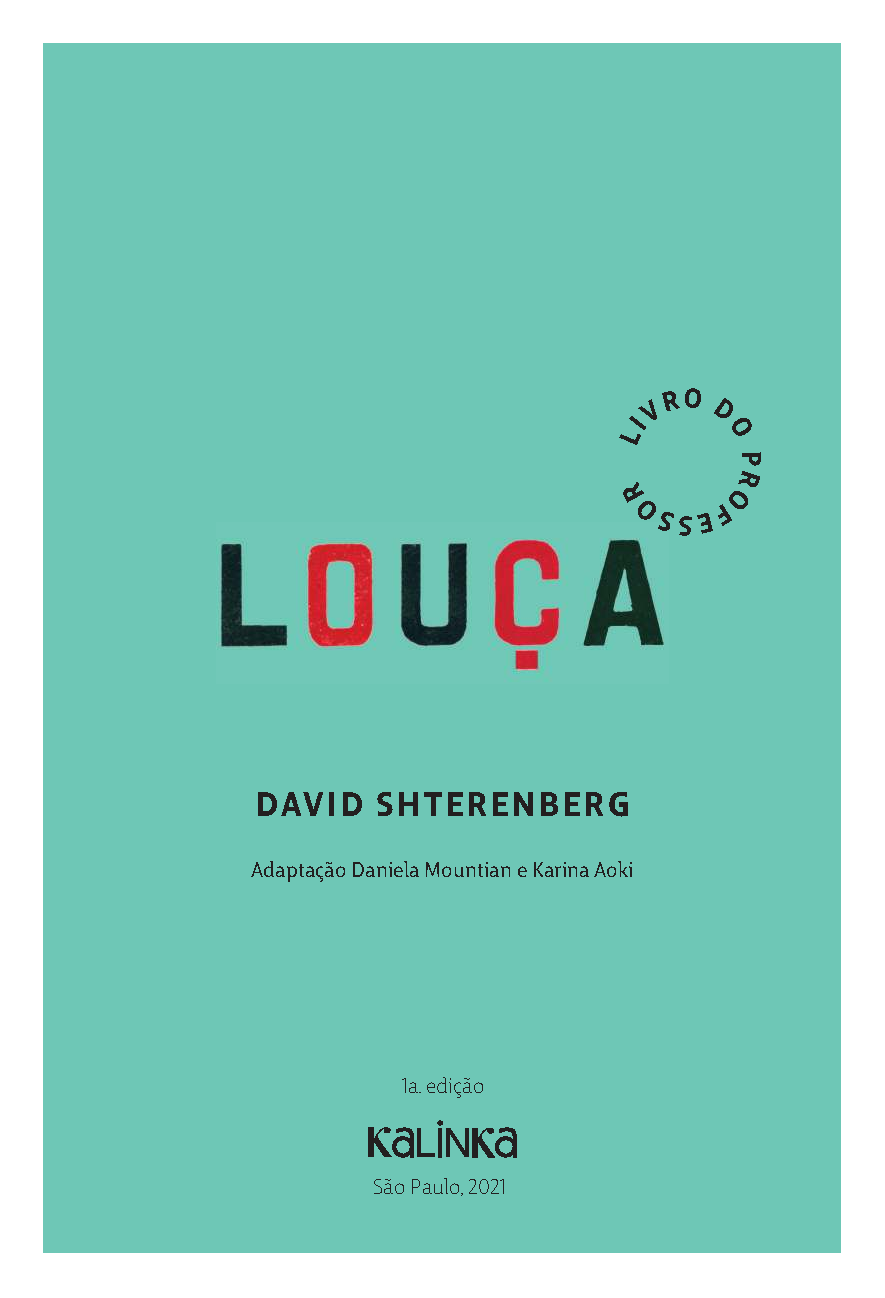
\includepdf[nup=2x2, 					% grid
			% offset=-15mm -5mm, 		% posição
			% scale=.8, 				% tamanho da página
            % delta=4mm 4mm, 			
            % frame,
            % pages={1-4}]{pdfs/PNLD2022-014_MIOLO.pdf}

\end{document}




